\section{Dispersion relations for concrete graph topologies} \label{sec:Examples}
In this section we want to include the following examples:
\begin{itemize}
	\item 1D chain with a single vertex (the ``simplest" decorator graph, which we discussed in the previous section), with coupling constants as zero coupling constants isn't that exciting
	\item The 2D-cross in plane example, with coupling constants. This is similar to the decorator case (at least in the dispersion relation which is derived), but could be used to show off some numerical results.
	\item (Potentially): A graph lacking symmetries, which requires a numerical treatment to find the eigenvalues?
\end{itemize}

Throughout this section, we are concerned with determining the spectrum of the problem \eqref{eq:WholeSpaceLaplaceEqn},
\begin{align*}
	-\laplacian_{\ddmes} u &= \omega^2 u, \quad\text{on } \reals^2,
\end{align*}
via determination of the spectrum of \eqref{eq:QGFullSystem},
\begin{align*}
	-\bracs{\diff{}{t} + i\qm_{jk}}^2 \tilde{u}_{jk} = \omega^2 \tilde{u}_{jk}, &\quad t\in\interval{I_{jk}}, \quad \forall I_{jk}\in \edgeSet, \\
	u \text{ is continuous at each } &v_j \in \vertSet, \\
	\sum_{j\con k}\bracs{\diff{}{t} + i\qm_{jk}}\tilde{u}_{jk}\bracs{v_j} = \alpha_j\omega^2 u\bracs{v_j}, &\quad \forall v_j \in \vertSet.
\end{align*}

\subsection{One-Dimensional ``Decorated" Loop} \label{ssec:Example1DLoop}
\tstk{brief intro for context}
Consider the graph $\graph$ periodic in one direction (WLOG parallel to the $x_1$-axis with $x_2=0$) in $\reals^2$, with vertices $v_j = \bracs{j + \recip{2}, 0}^\top$ and edges $I_{j\bracs{j+1}}$ for $j\in\integers$.
Assume the coupling constants at each vertex are identical, taking the value $\alpha\in\reals$.
Then the quantum graph which corresponds to the period graph of $\graph$ is simply a single vertex $v$ with a looping edge $I$ of length 1, with quasi-momentum $\qm$ on $I$ and coupling constant $\alpha$ at $v$. 
One can apply proposition \ref{prop:M-MatrixEntries} at this point to compute the (one-dimensional) ``$M$-matrix", however for illustrative purposes (and consistency with the examples that follow) we elect to introduce a dummy vertex to break the loop $I$ into two edges, producing a new quantum graph $\graph_{\mathcal{P}}=\mathcal{\vertSet, \edgeSet}$ with
\begin{align*}
	\vertSet = \clbracs{ v_1 , v_2 }, \quad &\edgeSet = \clbracs{ I_{12}, I_{21} }, \\
	\abs{I_{12}} = \abs{I_{21}} = \recip{2}, \quad &\qm_{12} = \qm_{21} = \qm, \\
	\alpha_1 = \alpha, \quad &\alpha_2 = 0.
\end{align*}
We illustrate the process of moving from $\graph$ to $\graph_{\mathcal{P}}$ in figure \ref{fig:Diagram_1DExample}.
Note that the dummy vertex having coupling constant equal to zero ensures that the incoming edge solutions and their derivatives match at $v_2$, ensuring that the introduction of $v_2$ does not alter the behaviour of solutions along the ``cut loop".
Studying the $M$-matrix of $\graph_{\mathcal{P}}$ to determine the eigenvalues $\omega^2$ is now equivalent to studying that of the original quantum graph we obtained.
\begin{figure}[t]
	\centering
	\begin{subfigure}[t]{0.3\textwidth}
		\centering
		\includegraphics[scale=2]{Diagram_1DLineGraph.pdf}
		\caption{\label{fig:Diagram_1DLineGraph} The graph $\graph$, periodic in one dimension, consisting of integer-spaced vertices.}
	\end{subfigure}
	~
	\begin{subfigure}[t]{0.3\textwidth}
		\centering
		\includegraphics[scale=2]{Diagram_1DLineQuantumGraph.pdf}
		\caption{\label{fig:Diagram_1DLineQuantumGraph} The corresponding quantum graph of the period cell of $\graph$, containing one (looping) edge of length 1}
	\end{subfigure}
	~
	\begin{subfigure}[t]{0.3\textwidth}
		\centering
		\includegraphics[scale=2]{Diagram_1DLineComputationGraph.pdf}	
		\caption{\label{fig:Diagram_1DLineComputationGraph} The equivalent graph $\graph_{\mathcal{P}}$ that we study. Note that the dummy vertex $v_2$ has coupling constant 0.}
	\end{subfigure}
	\caption{\label{fig:Diagram_1DExample} The graphs $\graph$ and $\graph_{\mathcal{P}}$.}
\end{figure} \newline

One can construct the $M$-matrix for $\graph_{\mathcal{P}}$ using proposition \ref{prop:M-MatrixEntries}, obtaining
\begin{align*}
	M_{\qm}\bracs{\omega} &= 
	\begin{pmatrix} 
		2\omega\cot\frac{\omega}{2} & -2\omega\csc\frac{\omega}{2}\cos\frac{\qm}{2} \\
		-2\omega\csc\frac{\omega}{2}\cos\frac{\qm}{2} & 2\omega\cot\frac{\omega}{2}
	\end{pmatrix}.
\end{align*}
Since the matrix of coupling constants $A = \mathrm{diag}\bracs{\alpha\omega^2, 0}$, we are required to work with the matrix
\begin{align*}
	\tilde{M}_\qm &= 
	\begin{pmatrix}
		2\omega\cot\frac{\omega}{2} - \alpha\omega^2 & -2\omega\csc\frac{\omega}{2}\cos\frac{\qm}{2} \\
		-2\omega\csc\frac{\omega}{2}\cos\frac{\qm}{2} & 2\omega\cot\frac{\omega}{2}		
	\end{pmatrix},
\end{align*}
and solve either $\tilde{M}_\qm\bracs{\omega} w = 0$, or $\det\tilde{M}_\qm \bracs{\omega} = 0$ for the eigenvalues $\omega^2$.
In this case, taking the latter approach is feasible analytically, and one can obtain the following equation for $\omega$ for a given $\qm$:
\begin{align*}
	\cos\qm &= \cos\omega - \frac{\alpha\omega}{2}\sin\omega.
\end{align*}
We would then need to determine the set of solutions for each $\qm\in\left[-\pi, \pi\right)$, and then taking the union would provide us with the spectrum of our original problem.
This procedure is similar to that in example \ref{ssec:ExampleCrossInPlane}, which we will study in greater depth, and so we forgo further analysis here.
However the methodology of example \ref{ssec:ExampleCrossInPlane} is applicable here, and as one might expect produces a spectrum of similar structure.

\subsection{Cross in the Periodic Plane} \label{ssec:ExampleCrossInPlane}
\tstk{intro sentence that provides relevance once we decide on the order to present the examples in}
Consider the periodic graph defined as follows; for each $\bracs{n,m}\in\integers^2$ define
\begin{align*}
	v_1^{\bracs{n,m}} = \bracs{\recip{2},0} + \bracs{n,m}, 
	&\quad v_2^{\bracs{n,m}} = \bracs{0,\recip{2}} + \bracs{n,m}, \\
	v_3^{\bracs{n,m}} = \bracs{\recip{2},\recip{2}} + \bracs{n,m}. & \\
	I_{13}^{\bracs{n,m}} = \sqbracs{v_1^{\bracs{n,m}}, v_3^{\bracs{n,m}}},
	&\quad I_{23}^{\bracs{n,m}} = \sqbracs{v_2^{\bracs{n,m}}, v_3^{\bracs{n,m}}}, \\
	I_{31}^{\bracs{n,m}} = \sqbracs{v_3^{\bracs{n,m}}, v_1^{\bracs{n+1,m}}},
	&\quad I_{32}^{\bracs{n,m}} = \sqbracs{v_3^{\bracs{n,m}}, v_2^{\bracs{n,m+1}}}.
\end{align*}
Then with 
\begin{align*}
	\vertSet^* &= \clbracs{v_j^{\bracs{n,m}} \ \vert \ j\in\clbracs{1,2,3}, \bracs{n,m}\in\integers^2}, \\
	\edgeSet^* &= \clbracs{I_{jk}^{\bracs{n,m}} \ \vert \ j,k\in\clbracs{1,2,3}, \bracs{n,m}\in\integers^2},
\end{align*}
and coupling constants
\begin{align*}
	\alpha_3^{\bracs{n,m}} &= \alpha \in\reals, \\
	\alpha_j^{\bracs{n,m}} &= 0, \quad j\in\clbracs{1,2,4,5},
\end{align*}
$\graph^* = \bracs{\vertSet^*,\edgeSet^*}$ is an embedded, periodic graph in $\reals^2$.
It's period graph occupies $\sqbracs{0,1}^2$ and can be visualised in figure \ref{fig:Diagram_TFRGraph}; consisting of 5 (although due to the association at the edges, effectively 3) vertices and 4 edges.
\begin{figure}[b!]
	\centering
	\begin{subfigure}[t]{0.45\textwidth}
		\centering
		\includegraphics[height=4.5cm]{Diagram_TFRGraph.pdf}
		\caption{\label{fig:Diagram_TFRGraph} The period graph that we are considering. All edges have length $\recip{2}$, and the quasi-momentum on horizontal edges is $-\qm_1$ and on vertical edges is $-\qm_2$.}
	\end{subfigure}
	~
	\begin{subfigure}[t]{0.45\textwidth}
		\centering
		\includegraphics[height=4.5cm]{Diagram_TFRQuantumGraph.pdf}
		\caption{\label{fig:Diagram_TFRQuantumGraph} The quantum graph that appears in our example in section \ref{ssec:ExampleCrossInPlane}. Due to the identification of vertices on the boundary of the period graph, we are effectively dealing with a 3-vertex quantum graph.}
	\end{subfigure}
	\caption{\label{fig:5VertexCross} (\ref{fig:Diagram_TFRGraph}) The period cell of the graph $\graph^*$. (\ref{fig:Diagram_TFRQuantumGraph}) The equivalent quantum graph on which we pose \eqref{eq:QGFullSystem}, retaining the lengths $l_{jk}$ and appropriate $\qm_{jk}$.}
\end{figure}
After associating the edges of the period graph, we obtain it's associated quantum graph $\graph=\bracs{\vertSet,\edgeSet}$ with $\vertSet=\clbracs{v_1,v_2,v_3}$, $\edgeSet=\clbracs{I_{13},I_{23},I_{31},I_{32}}$, and lengths
\begin{align*}
	l_{13} = l_{23} = l_{31} = l_{32} = \recip{2}.
\end{align*}
Given that all the edges of $\graph^*$ are parallel to the co-ordinate axes, it is also fairly easy to compute the values of $\qm_{jk}$ for each $I_{jk}\in E$ and a given $\qm=\bracs{\qm_1,\qm_2}\in[-\pi,\pi)^2$;
\begin{align*}
	\qm_{13} = \qm_{31} = -\qm_2, &\quad \qm_{23} = \qm_{32} = -\qm_1.
\end{align*}

We now look to determine the spectrum of the problem \eqref{eq:QGFullSystem}, to this end we use proposition \ref{prop:M-MatrixEntries} to write down the $M$-matrix:
\begin{align*}
	M_{\qm}\bracs{\omega} &=
	\begin{pmatrix}
		2\omega\cot\bracs{\frac{\omega}{2}} & 0 & -2\omega\csc\bracs{\frac{\omega}{2}}\cos\bracs{\frac{\qm_2}{2}} \\
		0 & 2\omega\cot\bracs{\frac{\omega}{2}} & -2\omega\csc\bracs{\frac{\omega}{2}}\cos\bracs{\frac{\qm_1}{2}} \\
		-2\omega\csc\bracs{\frac{\omega}{2}}\cos\bracs{\frac{\qm_2}{2}} & -2\omega\csc\bracs{\frac{\omega}{2}}\cos\bracs{\frac{\qm_1}{2}} & 4\omega\cot\bracs{\frac{\omega}{2}}
	\end{pmatrix}.
\end{align*}
At this point we have the option of solving for the spectrum numerically or analytically, however because we have such a small and symmetric problem we proceed analytically by solving $\mathrm{det}\bracs{ M_{\qm}\bracs{\omega} - A }=0$, where $A=\mathrm{diag}\bracs{0,0,\alpha\omega^2}$ is the matrix of coupling constants for $\graph$.
After some calculation,
\begin{align*}
	\det\bracs{\bracs{M_{\qm}\bracs{\omega} - \omega^2 A}} &= 0 \\
	\Leftrightarrow \cos\bracs{\frac{\qm_1+\qm_2}{2}}\cos\bracs{\frac{\qm_1-\qm_2}{2}} &= \cos\omega - \frac{\alpha\omega}{4}\sin\omega. \labelthis\label{eq:ExampleThickVertexSolution}
\end{align*}
For ease, we define
\begin{align*}
	\Xi\bracs{\omega, \wavenumber} := \cos\omega - \frac{\alpha\omega}{4}\sin\omega.
\end{align*}
The left hand side of \eqref{eq:ExampleThickVertexSolution} attains every value in the interval $\sqbracs{-1,1}$ over the range $\qm\in[-\pi,\pi)^2$, but the right hand side cannot be written as a function of $\omega$ alone.
So finding eigenvalues $\omega^2$ amounts to determining those $\omega$ for which
\begin{align} \label{eq:ExampleThickVertexDispExpr}
	-1 \leq \Xi\bracs{\omega} \leq 1.
\end{align}
One can visualise the curve $\Xi$ in figure \ref{fig:Scalar_ThickVertexDR}; and a numerical estimate of the density of states \tstk{we haven't defined this anywhere prior!} is provided in figure \ref{fig:CrossInPlane_DoS}.
\begin{figure}[t]
	\centering
	\begin{subfigure}[t]{0.45\textwidth}
		\centering
		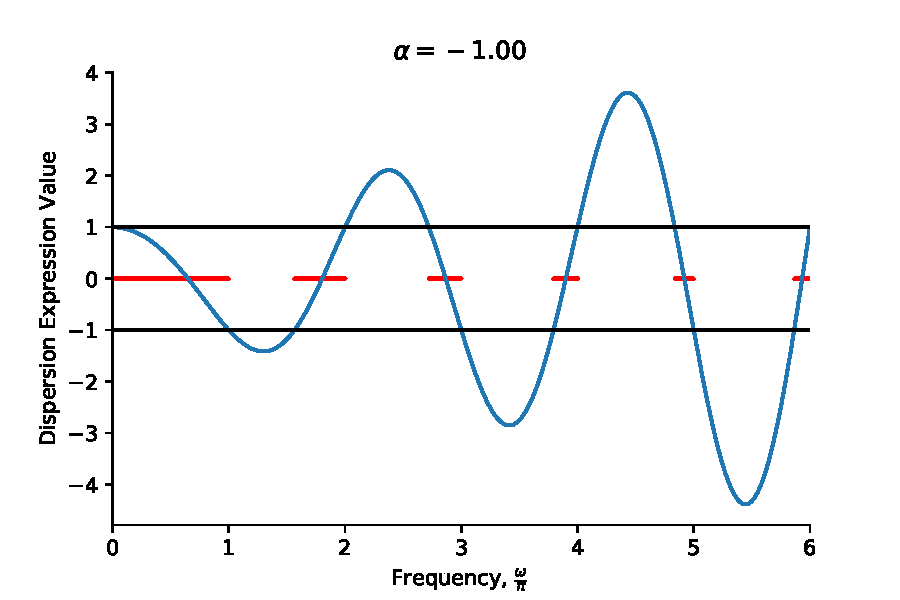
\includegraphics[scale=0.5]{Scalar_ThickVertexDR_a-1.pdf}
		\caption{\label{fig:Scalar_ThickVertexDR_a-1} The function $\Xi$ for $\alpha=-1$.}
	\end{subfigure}
	~
	\begin{subfigure}[t]{0.45\textwidth}
		\centering
		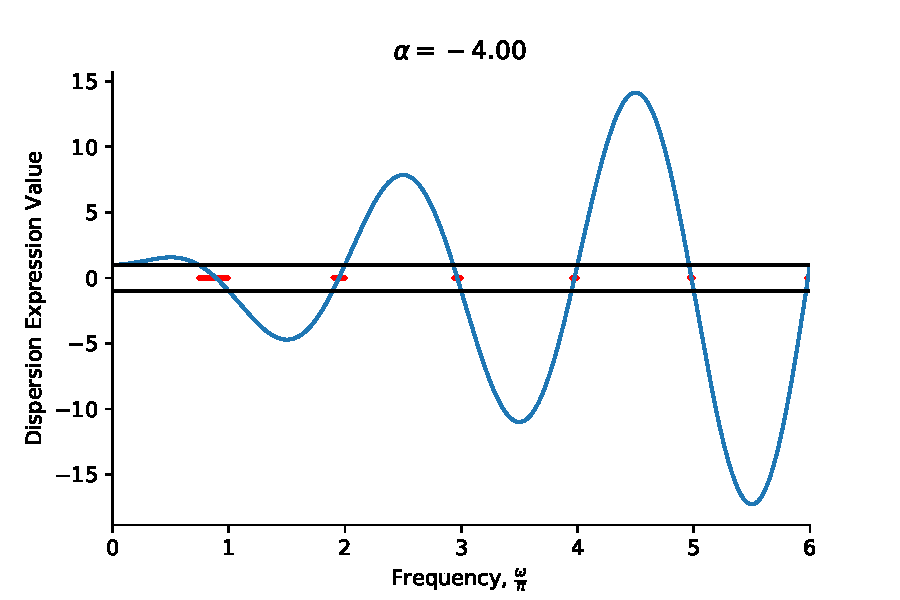
\includegraphics[scale=0.5]{Scalar_ThickVertexDR_a-4.pdf}
		\caption{\label{fig:Scalar_ThickVertexDR_a-4} The function $\Xi$ for $\alpha=-4$.}
	\end{subfigure}
	\caption{\label{fig:Scalar_ThickVertexDR} The function $\Xi$. Red regions indicate those $\omega$ that correspond to eigenvalues $\omega^2$, when $\Xi$ takes values between $-1$ and $1$ (black lines). One can see the existence of spectral bands which shrink in size as $\omega\rightarrow\infty$.}
\end{figure}
One can observe that the points $\omega$ that satisfy \eqref{eq:ExampleThickVertexDispExpr} are divided into distinct ``spectral bands" which shrink as $\omega\rightarrow\infty$.
\begin{figure}[b!]
	\centering
	\begin{subfigure}[t]{0.45\textwidth}
		\centering
		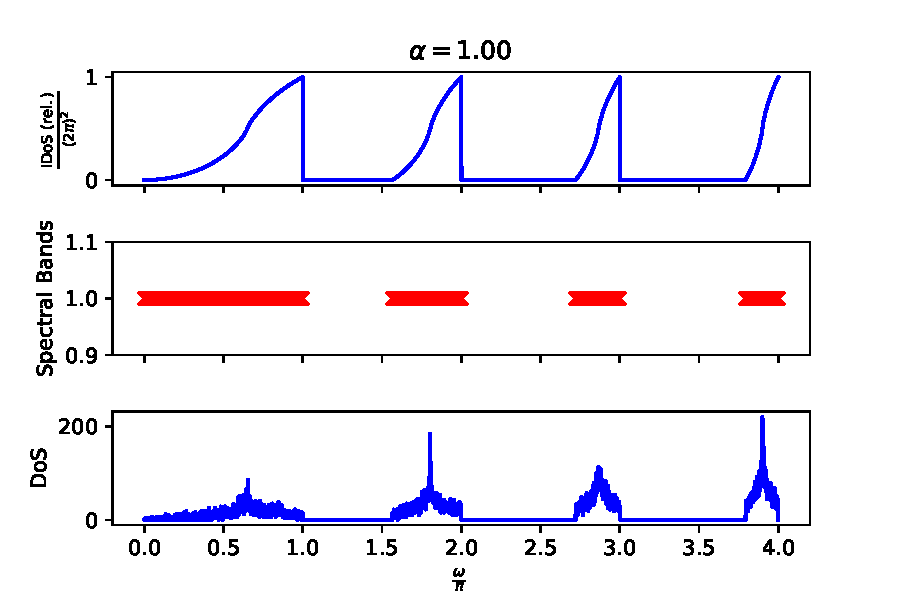
\includegraphics[scale=0.5]{CrossInPlane_DoS_Alpha1.pdf}
		\caption{\label{fig:CrossInPlane_DoS_Alpha1} The density of states and spectrum for the system with $\alpha=1$.}
	\end{subfigure}
	~
	\begin{subfigure}[t]{0.45\textwidth}
		\centering
		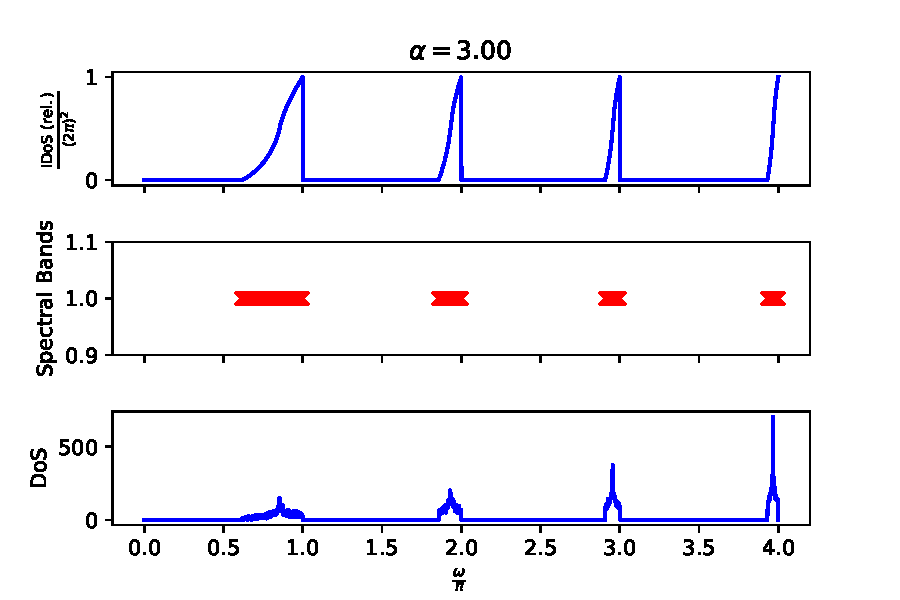
\includegraphics[scale=0.5]{CrossInPlane_DoS_Alpha3.pdf}
		\caption{\label{fig:CrossInPlane_DoS_Alpha3} The density of states and spectrum for the system with $\alpha=3$.}
	\end{subfigure}
	\caption{\label{fig:CrossInPlane_DoS} The spectrum and density of states for the graph topology in section \ref{ssec:ExampleCrossInPlane}.}
\end{figure}
The value of $\alpha$ affects whether there is a gap in the spectrum between 0 and the first spectral band, values of $\alpha<2$ result in the first band starting at 0, whilst $\alpha\geq 2$ results in a gap between zero and the bottom of the spectrum \tstk{do we want to give the results which validate the emergence of spectral bands? CF TFR.}.